\begin{figure}[htbp]
\centering
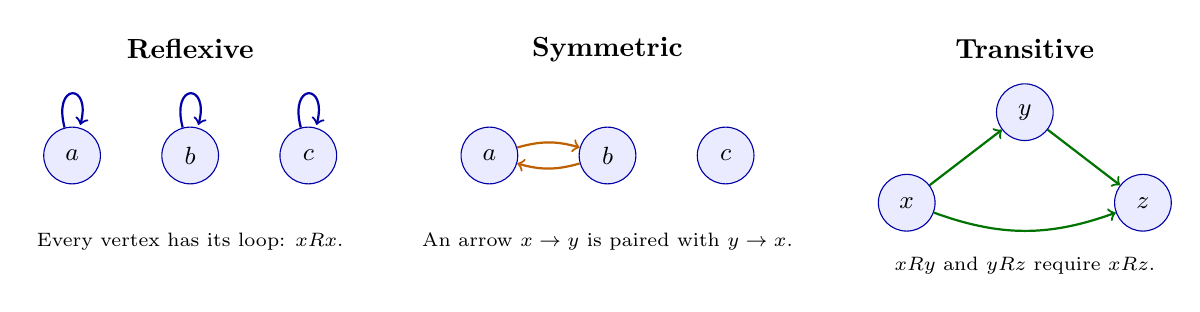
\begin{tikzpicture}[font=\small,vertex/.style={circle,draw=blue!65!black,fill=blue!8,minimum size=0.72cm}]
    \begin{scope}
        \node[font=\bfseries] at (2.3,2.7) {Reflexive};
        \node[vertex] (a) at (0.8,1.35) {$a$};
        \node[vertex] (b) at (2.3,1.35) {$b$};
        \node[vertex] (c) at (3.8,1.35) {$c$};
        \draw[->,thick,blue!65!black] (a) edge[loop above] (a);
        \draw[->,thick,blue!65!black] (b) edge[loop above] (b);
        \draw[->,thick,blue!65!black] (c) edge[loop above] (c);
        \node[align=center,font=\scriptsize] at (2.3,0.25) {Every vertex has its loop: $xRx$.};
    \end{scope}
    \begin{scope}[xshift=5.3cm]
        \node[font=\bfseries] at (2.3,2.7) {Symmetric};
        \node[vertex] (a) at (0.8,1.35) {$a$};
        \node[vertex] (b) at (2.3,1.35) {$b$};
        \node[vertex] (c) at (3.8,1.35) {$c$};
        \draw[->,thick,orange!75!black,bend left=16] (a) to (b);
        \draw[->,thick,orange!75!black,bend left=16] (b) to (a);
        \node[align=center,font=\scriptsize] at (2.3,0.25) {An arrow $x\to y$ is paired with $y\to x$.};
    \end{scope}
    \begin{scope}[xshift=10.6cm]
        \node[font=\bfseries] at (2.3,2.7) {Transitive};
        \node[vertex] (x) at (0.8,0.75) {$x$};
        \node[vertex] (y) at (2.3,1.9) {$y$};
        \node[vertex] (z) at (3.8,0.75) {$z$};
        \draw[->,thick,green!45!black] (x) -- (y);
        \draw[->,thick,green!45!black] (y) -- (z);
        \draw[->,thick,green!45!black] (x) to[bend right=20] (z);
        \node[align=center,font=\scriptsize] at (2.3,-0.05) {$xRy$ and $yRz$ require $xRz$.};
    \end{scope}
\end{tikzpicture}
\caption{Directed-graph patterns for the three defining properties of an equivalence relation. Each panel isolates one property; an equivalence relation must satisfy all three.}
\label{fig:relation-properties}
\end{figure}